\chapter{Introduction}
\label{sec:introduction}

\section{Thesis Overview}
\label{sec:overview}
This thesis performs a comparison of five feature extraction algorithms


Mobile Robot Localisation is defined as the ability of a mobile robot to determine its pose relative to a map of an environment \citep{Thrun2002}. Localisation is achieved by identifying landmarks in the environment and determining their corresponding positions on the map. The robot then uses this information to determine its pose. If a map of the environment is available, then the robot can immediately orient itself with respect to the map. However, in many cases a map is not available, in which case the robot has to first build a map of the environment and then localise using this map. This is referred to as Simultaneous Localisation and Mapping (SLAM) \citep{Durrant2006, Bailey2006b}.\\

In the past, identification of landmarks for the purposes of localisation and SLAM have been performed with laser-range finders and sonar sensors among others \citep{Davison2007}. Laser-range finder systems are usually accurate but slow whereas sonar sensors are fast and cheap but generate crude measurements \citep{Se2002}. On the other hand, vision systems such as cameras are of high resolution and are more intuitive since animals and humans heavily rely on this sense to navigate \citep{Davison2007}. In addition, vision systems are inexpensive and ubiquitous and therefore provide a feasible means for a robot to identify landmarks and subsequently localise itself in an environment.\\

The detection of visual landmarks (also referred to as \textit{Interest Points}) is achieved using feature extraction algorithms. A feature extraction algorithm utilises camera images to extract visual algorithmic-dependant interest points from the environment. These interest points can then be used as landmarks and a robot can then localise itself by subsequently re-observing these landmarks. \\

\begin{figure}[h!] 
  \centering
    \includegraphics[width=0.5\textwidth]{../Drawings/introduction/drcRobots.jpg}
    \caption{An artist's impression of the robots to be developed for the DARPA Robotics Challenge \citep{darpa2012}}
    \label{fig:darpa}
\end{figure}

\section{Motivation}
\label{sec:motivation}
The ability of a robot to localise itself with respect to its environment is crucial in many different applications. One of the more well-known applications is that of the Mars Rover used for space exploration. Due to a large communication latency, sending commands to the Mars Rover has a one-way data transfer time that varies between $6$ and $20$ minutes \citep{Powell2006}. Therefore, performing teleoperations to control the rover is impractical and often infeasible. The robot is therefore required to be autonomous which includes the ability to localise itself with respect to its environment such that it can identify landmarks, compute safe traversal paths and avoid obstacles \citep{Powell2006}.\\

Another application where localisation is of great importance is related to the \textit{DARPA Robotics Challenge} \citep{darpa2012}. The most recent challenge requires the development of robots for disaster-response operations. Often natural and man-made disasters create grave risks for rescue and aid workers that prevent a timely human response. Thus one potential solution is to deploy robots that can build maps and localise themselves in these environments and perform useful tasks such as clearing disaster sites and searching for victims as shown in \figref{fig:darpa}.\\   

\begin{figure}[h!] 
  \centering
    \includegraphics[width=0.5\textwidth]{../Drawings/introduction/drcRobots.jpg}
    \caption{An artist's impression of the robots to be developed for the DARPA Robotics Challenge \citep{darpa2012}}
    \label{fig:darpa}
\end{figure}

Using vision to perform localisation is highly desirable in a number of applications. Visual odometry has been used as a localisation technique on the Mars Rover \citep{Di2008} but since it requires a large amount of processing time, it can only be used in limited scenarios. This is in spite of the fact that visual odometry provides more accurate position estimation than previously used methods \citep{Powell2006}. Robots deployed to disaster zones can also benefit from vision systems for localisation. Here, the robot's ability to distinguish between different sides of a room or building as well as uniquely identify specific regions within the disaster zone is of great importance in these dynamic environments. In principle, vision systems could potentially be used to localise robots that are exploring suburbs and cities. If a robot can uniquely identify visual landmarks whilst in a specific street, then it can in principle determine its location by comparing these visual landmarks to a database of visual landmarks coupled with predefined locations. An image database such as Google Street View could be used for this purpose \citep{StreetView}.\\

Performing localisation using a vision system faces a number of difficult challenges. The first main challenge is identifying stable visual landmarks that do not vary significantly over time \citep{Davison2007, Se2002}. In addition to this, the same landmarks may be re-observed from different scales, orientations and translations \citep{Szeliski2010}. Thus, depending on the domain, the landmarks need to be invariant to some or all of these changes. Visual landmarks may also suffer from occlusion and varying lighting conditions, which may prevent the landmark from being re-observed. Finally, perhaps the most crucial aspect of visual landmark localisation is that the image processing algorithms required to identify the landmarks can be computationally expensive \citep{Juan2009}. In addition to this, many mobile robots have significant resource constraints that require a computationally efficient visual processing algorithm \citep{NaoHead}. \\

\subsection{Application Domain}
\label{sec:domain}
An immediate domain for using a vision system to identify landmarks and perform localisation is the Robocup competition. Robocup is a robot football competition that was set up in 1997 in order to advance research in Artificial Intelligence (AI) and Robotics \citep{Robocup}. The original goal of the Robocup competition was to field a team of robots that would be able to defeat the human football world champions by the year $2050$.\\

There are a number of different leagues in which different types of robots compete. The Nao humanoid robot, which is the robot that will be used for this project, currently competes in the Standard Platform League \citep{StandardPlatform}.\\

The general setup of a Robocup game of football in the Standard Platform League is shown in \figref{fig:naofield}. There are four robots per team which include one goalkeeper and three outfield players \citep{Rules}. The aim of the game is to score more goals than the opponent using a Mylec orange street hockey ball by kicking the ball into the opponent's goal.\\

%Identify common methods applied in the field and voids in literature
\begin{figure}[h!] 
  \centering
    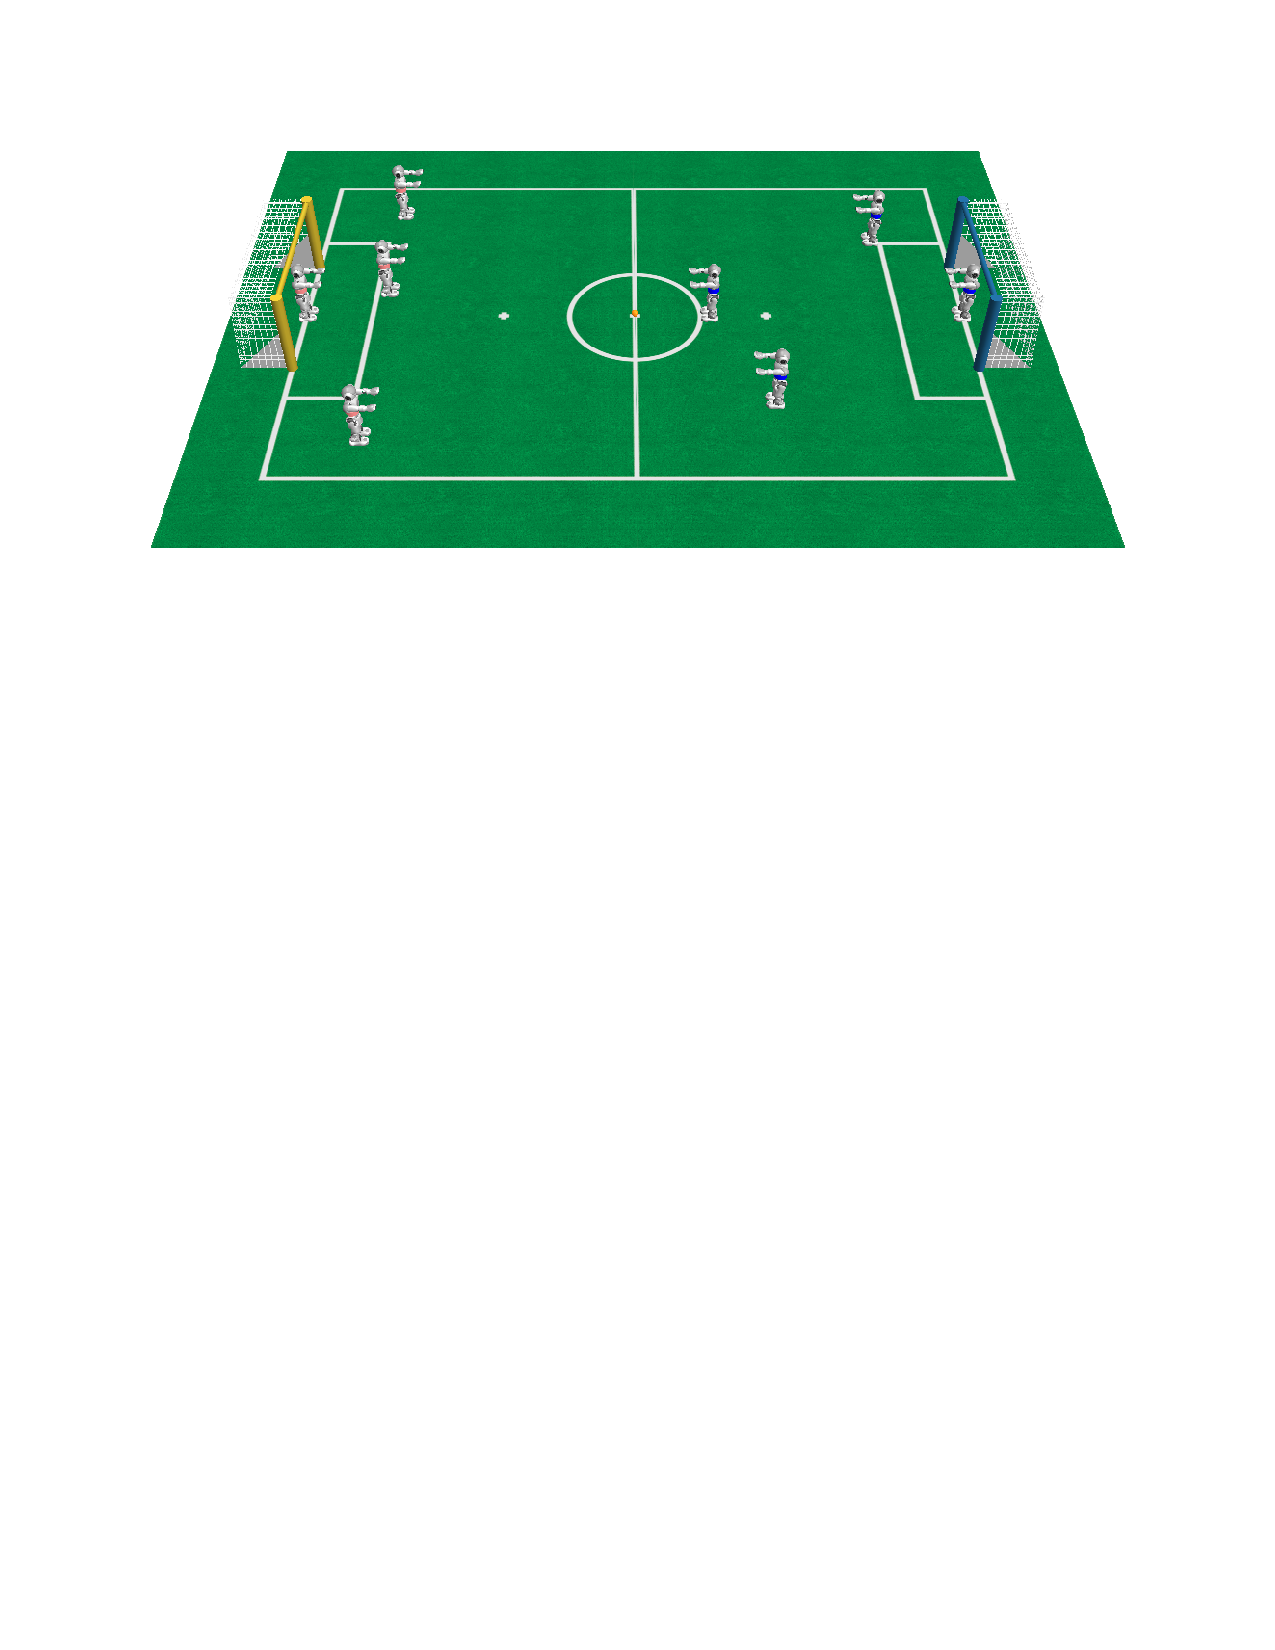
\includegraphics[width=0.8\textwidth]{../Drawings/robocup/NaoField.jpg}
    \caption{The standard setup for a game of football before kick-off \citep{Rules}}
    \label{fig:naofield}
\end{figure}

This year, the Robocup environment has incorporated a significant modification. The goal posts, which were previously yellow and blue for each team respectively, will now be the same colour. This means that the robot will be unable to disambiguate between its side of the field and that of its opponents due to the symmetrical nature of the environment as shown in \figref{fig:naofield}. This makes it difficult for the robot to localise itself relative to the field.\\

This recent modification to the Robocup has created the opportunity to determine whether the Nao's vision system can be used to identify visual landmarks that are found outside of the field. These landmarks can then be used to localise the Nao's position on the football field. This is a useful domain since many of the problems inherent to disaster zones and the Mars rover are also apparent in the Robocup competition. These include ambiguities due to the symmetrical nature of the environment as well as the dynamics of the environment such as humans and other robots potentially occluding the visual landmarks.\\

\subsection{The Nao's Vision System}
\label{sec:naoSpecs}
The Nao robot to be used for the project will use the latest Nao head, Head $4.0$, that has been designed by Aldebaran Robotics \citep{NaoHead}. The specifications for the new Nao head are shown in \figref{fig:nao1} and \figref{fig:nao2} respectively. The Nao's head incorporates a vision system that will be used to identify visual landmarks to be used for localisation.\\

The Nao's vision system consists of two cameras that are placed vertically above one another. These cameras provide a $640 \times 480$ resolution and operate at $30$ frames per second (fps). These cameras operate in the \textit{YUV422} colour space.\\

It is important to note that the vertical field of view has been increased for each of the cameras respectively to $47.64^\circ$ which may make it possible to detect features on the ceiling above the Robocup field. In addition to this wider field of view, the robot has a yaw range of $-119.5^\circ$ to $119.5^\circ$ and a pitch range of $-38.5^\circ$ to $29.5^\circ$ as shown in \figref{fig:yawPitch}.\\ 

 \begin{figure}[ht!]
\begin{minipage}[b]{0.6\linewidth}
  \centering
    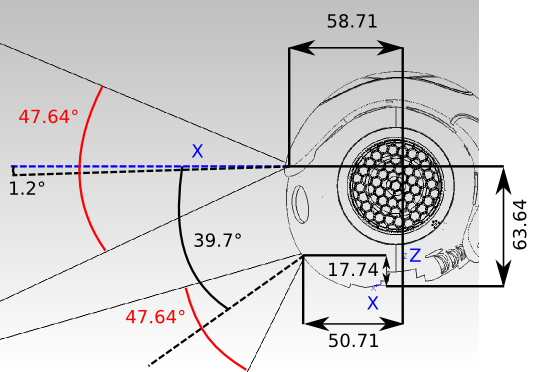
\includegraphics[width=0.6\textwidth]{../Drawings/naoHead/naoHead.jpg}
    \caption{A side view of the new Nao head \citep{NaoHead}} 
    \label{fig:nao1}
\end{minipage}
\begin{minipage}[b]{0.6\linewidth}
  \centering
    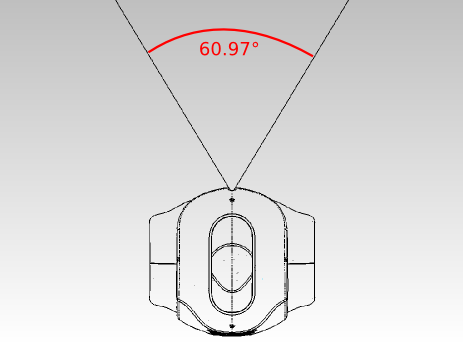
\includegraphics[width=0.6\textwidth]{../Drawings/naoHead/naoHead1.jpg}
    \caption{A top view of the new Nao head \citep{NaoHead}} 
    \label{fig:nao2}
\end{minipage}
\end{figure}

\begin{figure}[h!] 
  \centering
    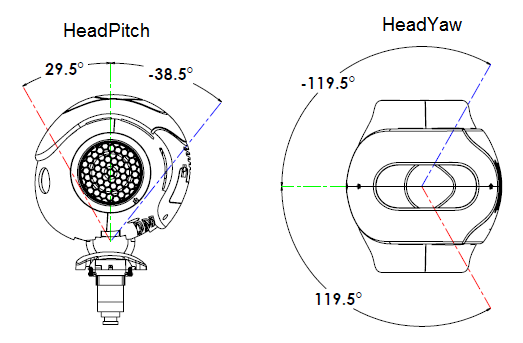
\includegraphics[width=0.5\textwidth]{../Drawings/naoHead/headyawpitch.png}
    \caption{The yaw and pitch of the Nao head \citep{NaoHead}} 
    \label{fig:yawPitch}
\end{figure}


%A landmark that has been identified using a visual perception system is often referred to as an \textit{interest point}. One popular definition of an interest point is a specific location or patch in an image that has a large contrast change with respect to its neighbors \citep{Szeliski2010}. Examples include edges and corners in images.\\
\section{Main Objectives}
\label{sec:objectives}
This thesis conducts a comparison of five different feature extraction algorithms in terms of computational performance and matching accuracy. Matching accuracy refers to the ability of an algorithm to correctly match a pair of images that contain the same visual landmarks. Image datasets are generated using the Nao's camera and the algorithms are compared for this data. The algorithm with the best performance along these dimensions is then further analysed and is recommended as the algorithm to be implemented on the Nao robot. In addition to this, a novel localisation algorithm has been developed for the purposes of Robocup. This algorithm aims to incorporate the best performing feature extraction algorithm to enable the Nao robot to localise itself on the football pitch.\\


%Localisation is where an agent is given a map of the environment and needs to determine its position relative to the map. This can be achieved be forming hypotheses of possible positions and weighting the likelihood of being in a certain position based on observations of the environment. If an agent is removed from the environment (the so-called \textit{kidnapping} problem) then it has to re-establish its position relative to the map. In a symmetrical environment, such as a football field, this can be difficult since the robot can be in a number of possible locations on re-entering the football field. In this case, it may be possible to solve the problem by observing visual natural features that are found above the football field.\\
%
%This is a difficult task since the features may be dynamic as a result of changes in illumination. It is also possible that the robot's visual system may not observe the same features based on its location on the pitch. The robot also has limited processing capabilities and thus processing constraints are placed on the possible algorithms. \\
%
%This problem is important since disambiguating a robot's location in an environment, based on observing distinct visual natural features, can create a generic localisation technique that can be extended to more general situations. These include rescue missions and household chores where a robot's ability to determine its location is crucially based on observing distinct visual natural features. An in-depth description of the proposal for solving this task will be described in the sections to follow.\\ 
%
%What is the problem?
%
%Why is it important?
%
%Why is it difficult?

%What is my hypothesis?

\section{Related Work}
\label{sec:relatedWork}
There are a number of different works that utilise feature extraction algorithms to detect visual landmarks and perform robot localisation. One of the first feature extraction algorithms is called the Scale Invariant Feature Transform (SIFT)\citep{Lowe2004}. This algorithm detects landmarks that are invariant to translation, rotation and image scaling and are thus ideal for a situation where features may be detected from multiple views. A Monte Carlo Localisation algorithm has been implemented using SIFT for feature detection \citep{Gil}. The robot is given a map of the environment and, using stereo vision, is able to find its location in an environment with better accuracy compared to using odometry estimates.\\


SIFT has been implemented on various different SLAM implementations. Using a triclops stereo vision system and detecting visual landmarks using SIFT, a mobile robot has been able to perform homing with good accuracy \citep{Se2001, Se2002}. The visual landmarks detected using SIFT were robustly matched and a consistent 3-dimensional map was generated. SIFT has also been implemented on a mobile robot, with a stereo camera and odometric sensors, using a FastSLAM algorithm. It achieved very good feature tracking and enabled the robot to estimate its position to within $0.5\%$ to $4\%$ of the total distance travelled \citep{Barfoot2005}.\\

SIFT and a variation of SIFT, called Speeded-Up Robust Features (SURF) \citep{Bay2008}, have been utilised for underwater SLAM \citep{Aulinas2011, Thomas}. The work conducted by \citet{Aulinas2011} extracts features from underwater images using SURF and matches the features using the SURF matching algorithm. This is performed off-line but results in increased accuracy in the final SLAM estimate.\\

Single camera SLAM, more formally referred to as Monocular SLAM (MonoSLAM), has also been utilised to good effect. Davison \textit{et al.} \citep{Davison2007} uses a single uncontrolled camera as the sole sensor on a mobile robot to actively perform localisation and mapping. The algorithm detects persistent natural features in the environment and is also able to determine the orientation of the features. MonoSLAM has also been implemented on a humanoid robot \citep{Wang2011}. SURF was used as the feature detection technique and visual SLAM was achieved.\\

Regarding the Robocup, one previous work has been developed by the \textit{rUNSWift} Robocup team to enable a Nao robot to localise itself on the Robocup football pitch using visual landmarks \citep{Anderson}. Visual landmarks are detected along a single row of pixels. This is achieved using 1D SURF, a variation of 2D SURF, that has been developed to detect and match interest points along this single dimension \citep{Anderson}. 1D SURF is significantly faster than 2D SURF and has been implemented in real-time on a robot.\\

%There are a number of algorithms currently available such as the Scale Invariant Feature Transform (SIFT)\citep{Lowe2004}. This algorithm detects features that are invariant to translation, rotation and image scaling and are thus ideal for a situation where features may be detected from multiple views. A far faster yet slightly less robust version of SIFT is Speeded-Up Robust Features (SURF) \citep{Bay2008}. This method maintains good performance compared to SIFT as well as other feature detection techniques \citep{Juan2009} and is ideal for systems that are constrained by the amount of processing power available. Another newer and potentially faster feature detection algorithm is that of Binary Robust Invariant Scalable Keypoints (BRISK) \citep{Leutenegger2011}. This approach utilises a scale-space FAST-based detector and outperforms the original, unmodified version of SURF by an order of magnitude in the experiments conducted in \citep{Leutenegger2011}.



%(For both appraoches describe stereo vision or monocular vision solutions)
%SLAM-based approaches




%Localisation-based approaches


%1. What other work has been done involving localisation using natural visual landmarks
%1.1 Start by describing localisation using stereo vision.
%1.2 Then describe localisation using a single camera

%2. What have the rUNSWift team achieved using natural visual landmarks.

%The above-mentioned feature detection techniques are used to detect features in the robot's environment. These features are the observations that are fed into localisation as well as Simultaneous Localisation and Mapping (SLAM) algorithms. The observed features are detected and their range and bearing measured either using stereo vision, involving two or more cameras, or using a single camera and various specialised feature-detection techniques.\\

%
%Single camera SLAM, more formally referred to as Monocular SLAM (MonoSLAM), has also been utilised to good effect. Davison \textit{et al.} \citep{Davison2007} uses a single uncontrolled camera as the sole sensor on a mobile robot to actively perform localisation and mapping. The algorithm detects persistent natural features in the environment and is also able to determine the orientation of the features. MonoSLAM has also been implemented on a humanoid robot \citep{Wang2011}. SURF was used as the feature detection technique and visual SLAM was achieved.\\




\section{Outline}
\label{sec:outline}
The structure of the thesis is as follows: Chapter \ref{sec:background} gives an in-depth overview of the main feature extraction techniques that have been used in this project. These include 2D SURF and Binary Robust Invariant Scalable Keypoints (BRISK). Chapter \ref{sec:realtimeFeatureExtraction} discusses the variations of these methods that have been developed for the purposes of Robocup. This Chapter also includes a discussion of the \textit{rUNSWift} team's 1D SURF feature extraction algorithm. Chapter \ref{sec:matching} details the matching techniques and constraints that have been implemented and developed respectively to match interest points in corresponding images. This is followed in Chapter \ref{sec:localisation} by a description of the localisation algorithm that has been developed for the Nao Robot to use in the Robocup competition. Chapter \ref{sec:experimentsResults} contains the results obtained from comparing the various feature extraction algorithms in a number of different environments. The best performing algorithm is then recommended and analysed further. Finally, Chapter \ref{sec:Conclusion} concludes the thesis by discussing potential problems, limitations and recommendations for future work. The key results are also summarised.\\